\documentclass{beamer}

\mode<presentation>
{
  \usetheme{EastLansing}      
  \usecolortheme{crane} 
  \usefonttheme{structurebold}  
  \setbeamertemplate{navigation symbols}{}
  \setbeamertemplate{caption}[numbered]
} 

\usepackage[utf8]{inputenc} 
\usepackage[T1]{fontenc} 
\usepackage[turkish,shorthands=:!]{babel} 
\usepackage{minted} 
\usepackage{hyperref} 

\title[Sunum]{Bilgisayar Mühendisliği Semineri Dersi \newline 3D Modelleme Sunumu} 
\author[D. E. K. \& E. N. K. \& S. A.]{ \inst{1} Name1 \and  \inst{2} Name2 \and  \inst{3} Name3} 
\institute[Bilgisayar Müh.]{\inst{1} No1 \and \inst{2} No2\and  \inst{3} No3 } 
\date{25.05.2022}

\begin{document}

\begin{frame}
  \titlepage
\end{frame}

\begin{frame}{Outline}
  \tableofcontents
\end{frame}

\section{Giriş}

\begin{frame}{Giriş}

\begin{itemize}
  \item Yapısal kalp hastalığı (SHD), kardiyovasküler tıpta yeni bir alandır. 
  \item Geleneksel görüntüleme yöntemleri hastalık teşhisi kavramı etrafında yapılandırıldıkları için, SHD müdahalelerinin ihtiyaçlarını desteklemekde yetersiz kalmaktadır.
  \item SHD müdahaleler, görüntülemenin prosedür içi planlamasını, simülasyonunu ve tahmin edilmesini gerektiren geleneksel görüntüleme kavramlarını bozar. 
  \item Klinik bakım ve prosedür planlamasında 3 boyutlu (3D) baskının uyarlanması, transkateter müdahaleler için erken teşhiste önemlidir. 
  \item Hesaplama modellemenin 3D'ye entegrasyonu baskı, cihaz testinde akışkanlar mekaniğinin araştırma ve geliştirme anlayışını hızlandırdı. 
  \item 3D baskı, hesaplamalı modelleme ve nihayetinde yapay zekanın dahil edilmesi, sağlık uygulamalarının seyrini değiştirdi.  
\end{itemize}

\end{frame}

\section{3D BASKI, BİLGİSAYARLI MODELLEME VE AI'NIN TEMELLERİ}

\subsection{3D MODELLEME NEDİR?}

\begin{frame}[allowframebreaks]{3D MODELLEME NEDİR?}

\begin{itemize}
    \item Üç boyutlu modelleme "hızlı prototipleme veya eklemeli imalat" olarak adlandırılan bir üretim tekniğidir. 
    \item Bu süreç, dijital olarak tanımlanmış geometriler üzerine çok sayıda malzeme katmanı yerleştirerek dijital nesneleri 3D fiziksel kopyalara dönüştürür. 
    \item Üç boyutlu basılı modelleme, bir dizi ardışık adımdan oluşan çok aşamalı bir süreçtir. 
    \item Hastaya özel 3D baskılı modelin üretilmesi, yüksek kaliteli görüntüleme verilerinin alınması ve bunun daha ileri görüntü işleme için uygun bir “Dijital Görüntüleme ve Tıpta İletişim (DICOM)” formatına dönüştürülmesiyle başlar. 
    \item DICOM görüntüleri daha sonra, segmentasyon adı verilen bir süreçte ilgilenilen anatomik vücut parçalarını tanımlamak ve oluşturmak için özel görüntü işleme yazılımına aktarılır. 
    \item Segmentasyonu, 3D hacim oluşturma ve hastaya özel geometrilerin dijital modellemesi takip eder. 
    \item Hastaya özel 3D dijital anatomik modeller, 3D baskıya uygun karmaşık geometrilerin yüzey ağ bilgilerini içeren stereolitografi (STL) dosya formatlarında kaydedilir ve bilgisayar destekli tasarım modellemesi ve hesaplamalı analiz yoluyla ek iyileştirmelere izin verir.
\end{itemize}

\end{frame}

\subsection{3D BASKI TEKNOLOJİLERİNE GENEL BAKIŞ}

\begin{frame}[allowframebreaks]{3D BASKI TEKNOLOJİLERİNE GENEL BAKIŞ}

\begin{itemize}
    \item Stereolitografi (SLA), 1980'lerde geliştirilen ilk 3D baskı teknolojisiydi. 
    \item Işığa duyarlı bir sıvı reçine olan temel malzemeyi katman katman bir şekilde işlemek için ultraviyole (UV) lazer kullanır ve 3D bir parça üretir.
    \item Tasarım gereği, SLA bir modelde yalnızca 1 malzeme kullanabilir. 
    \item Çoğu durumda, daha sonra çıkarılması gereken ekstra destekleyici yapıları yazdırması gerekir. 
    \item SLA, eğitim, öğretim ve akış testi için kardiyak ve vasküler modeller gibi büyük, yüksek doğrulukta ve şeffaf modeller üretmek için idealdir. 
    \item Seçici lazer sinterleme (SLS), naylon, metal ve seramik gibi ısıya duyarlı malzemelerin küçük parçacıklarının katmanlarını birleştirmek için yüksek güçlü kızılötesi lazer kullanan bir teknolojidir. 
    \item SLS, kardiyovasküler uygulamalarda yaygın olarak değil, çoğunlukla imalat sanayinde kullanılmaktadır. 
    \item Birleştirilmiş biriktirme modellemesi (FDM), evde veya ofiste masaüstü kullanımına uygun, nispeten düşük maliyetli bir teknolojidir. 
    \item Bir termoplastik filamentin veya metal telin küçük parçalarını eritir ve ekstrüde ederek bunları katmanlar halinde biriktirir. 
    \item FDM, nispeten düşük bir bütçeyle sert ve güçlü modeller üretmek için idealdir.
    \item Mürekkep püskürtmeli 3D baskı teknolojisi, 2D mürekkep püskürtmeli yazıcıya benzer şekilde çalışır. 
    \item Tam renkli bir 3D nesne oluşturmak için toz katmanlarını birleştirmek ve katılaştırmak için küçük renkli sıvı bağlayıcı damlacıkları biriktirir. 
    \item Inkjet yalnızca tek bir temel malzeme kullanabilir. 
    \item Son olarak, Stratasys (Rehovot, İsrail) tarafından geliştirilen Polyjet teknolojisi, bir dereceye kadar SLA ve inkjet teknolojilerinin bir birleşimidir. 
    \item Bir 3D nesne üretmek için UV ile işlenebilen fotopolimerleri katmanlar halinde biriktirir. 
    \item 2 veya daha fazla baz malzemeyi karıştırarak, çok çeşitli renk ve fiziksel özelliklere sahip “dijital malzemeler” ile baskı yapabilir. 
    \item Polyjet, son zamanlarda kalsifik lezyonlu aort kökü gibi sert parçaları olan uyumlu kardiyovasküler modelleri yazdırmak için kullanılmıştır. 
\end{itemize}

\end{frame}

\begin{frame}{}
\begin{block}{}
\includegraphics[width=12cm,height=8cm]{Şekil 1.jpg}
\end{block}
\end{frame}

\subsection{VERİ BÖLÜMLEME VE GÖRÜNTÜ OLUŞTURMA İLKELERİ}

\begin{frame}{VERİ BÖLÜMLEME VE GÖRÜNTÜ OLUŞTURMA İLKELERİ}

\begin{itemize}
    \item Medikal görüntülerde ilgili kalp bileşenlerinin sınırlarının çizilmesi işlemine genellikle görüntü segmentasyonu denir. 
    \item Kalbin hesaplamalı modellemesinde ilk ve genellikle en yoğun emek gerektiren adımdır. 
    \item SHD'li hastalarda elde edilen hacimsel DICOM görüntülerini işlemek için özel 3D segmentasyon ve modelleme yazılımı geliştirilmiş ve kullanılmıştır. 
    \item Hesaplamalı modellemede kullanılan kardiyak dokuların materyal özellikleri esas olarak hayvan dokuları ve/veya insan kadavraları üzerinde yapılan in vitro biyomekanik testlerden elde edilir. 
\end{itemize}

\end{frame}

\begin{frame}{}
\begin{block}{}
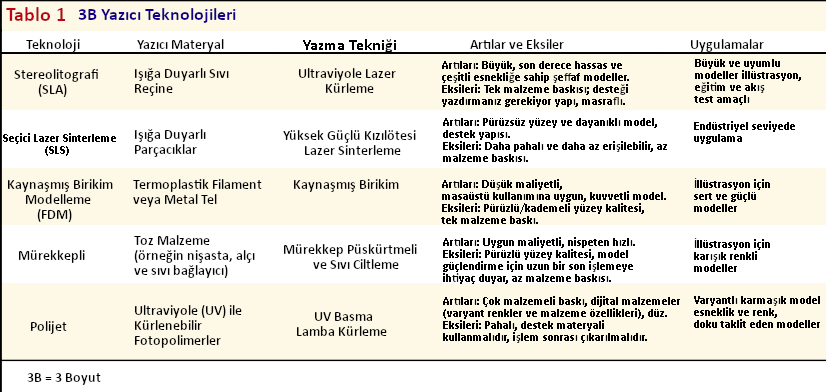
\includegraphics[width=12cm,height=8cm]{Tablo 1.png}
\end{block}
\end{frame}

\begin{frame}{}
\begin{block}{}
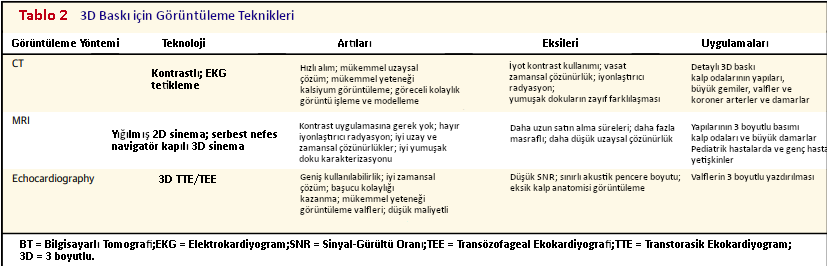
\includegraphics[width=12cm,height=8cm]{Tablo 2.png}
\end{block}
\end{frame}

\subsection{TRANSKATETER MİTRAL KAPAKÇIK DEĞİŞİMİ İÇİN 3D BASKI VE SANAL SİMÜLASYON}

\begin{frame}{TRANSKATETER MİTRAL KAPAKÇIK DEĞİŞİMİ İÇİN 3D BASKI VE SANAL SİMÜLASYON}

\begin{itemize}
    \item Transkateter mitral kapak replasmanında (TMVR), "neo"-LVOT'nin (sol ventriküler çıkış yolu) anlaşılması, çıkış obstrüksiyonu riski taşıyan ilgili LVOT anatomisinin hastaya özel 3D baskısında cihazların masaüstü simülasyonu ile başladı. 
    \item Fiziksel 3D baskı, bir iletişim aracı ve TMVR cihazı iniş bölgesinin hastanın mitral düzleminde nerede olacağının görsel testi ve TMVR sonrası neo-LVOT'un ne kadar küçük olacağının görsel bir değerlendirmesi olarak hizmet etti.
    \item Hastalarda TMVR öncesi ve sonrası prosedürel BT'ler elde edildikten sonra, neo-LVOT kavramı, fiziksel 3D baskıdan sanal 3D baskı kapakçık implantasyonuna ve ilgili trans kateter cihazlarıyla simülasyona geçebildi.
\end{itemize}

\end{frame}

\begin{frame}{}
\begin{block}{}
\includegraphics[width=12cm,height=8cm]{Şekil 2.jpg}
\end{block}
\end{frame}

\begin{frame}{}
\begin{block}{}
\includegraphics[width=12cm,height=8cm]{Şekil 3.jpg}
\end{block}
\end{frame}

\section{3D BASKININ GÜNCEL KISITLAMALARI}

\begin{frame}{3D BASKININ GÜNCEL KISITLAMALARI}

\begin{itemize}
  \item İdeal olarak, 3 boyutlu basılmış bir kardiyovasküler model, canlı organın hem görünümünü hem de mekanik özelliğini taklit etmelidir. 
  \item In vitro cihaz testi ve/veya prosedür simülasyonu için, tercihen 3D baskılı model aynı zamanda bir kalp döngüsü boyunca hedef kardiyovasküler organın dinamik davranışını da taklit etmelidir ancak bu materyallerin biyolojik dokuların doğrusal olmayan ve anizotopik davranışlarını taklit etmedeki yetersizlikleri nedeniyle biyolojik dokulara mükemmel şekilde uyan materyalleri bulmak hala zordur. 
  \item Bu tür teknolojiler henüz emekleme aşamasındadır ve yüksek düzeyde aktif kuvvet uygulayan hızlı atan bir kalbi simüle etmek için uygun değildir. 
\end{itemize}

\end{frame}

\section{3D BASKININ ÖTESİNDE: BİLGİSAYARLI MODELLEME VE AI'NİN TEMELLERİ}

\begin{frame}{3D BASKININ ÖTESİNDE: BİLGİSAYARLI MODELLEME VE AI'NİN TEMELLERİ}

\begin{itemize}
  \item Statik 3D baskılı modeller, hızlandırılmış süreç araştırma ve geliştirme ekiplerinin şu anda yeni cihaz konseptinden perkütan solüsyonların klinik ortama ulaştırılmasına kadar geçen süreyi azaltmak için başvurduğu bir yöntemdir. 
  \item Statik baskılar, perkütan kalp kapakçık cihazları ve uygulama sistemleri ,ideal test ortamını simüle etmek için hastaya özel basınçlı hemodinamik koşullar altında işlevsel 3D baskılı modellere dönüşmüştür. 
  \item Hesaplamalı simülasyon genellikle sonlu elemanlar analizi (FEA) ve hesaplamalı akışkanlar dinamiği (CFD) gibi sayısal analiz yöntemleri kullanılarak gerçekleştirilir. 
\end{itemize}

\end{frame}

\begin{frame}{}
\begin{block}{}
\includegraphics[width=12cm,height=8cm]{Şekil 4.jpg}
\end{block}
\end{frame}

\section{TEKNOLOJİDE AŞILMASI GEREKEN ZORLUKLAR}

\begin{frame}{TEKNOLOJİDE AŞILMASI GEREKEN ZORLUKLAR}

\begin{itemize}
  \item Yapay zekanın gerçek dünyadaki uygulamasındaki ana zorluk, büyük miktarda yapılandırılmamış klinik verinin varlığıdır. 
  \item Veri toplamanın temel taşı, uygun kaynak görüntü biçimlendirmesi, sunucular arasındaki dosya dönüşümlerinin uyumluluğu ve doğrudan öğrenme bulutuna yükleme yeteneğidir. 
  \item Yüklenen veriler buluttaki mevcut veri kümelerine dahil edildikten sonra, daha yalın süreçler oluşturmak için yeni veriler kullanıldıkça AI algoritmaları etkinleştirilecek ve geliştirilecektir. 
\end{itemize}

\end{frame}

\begin{frame}{}
\begin{block}{}
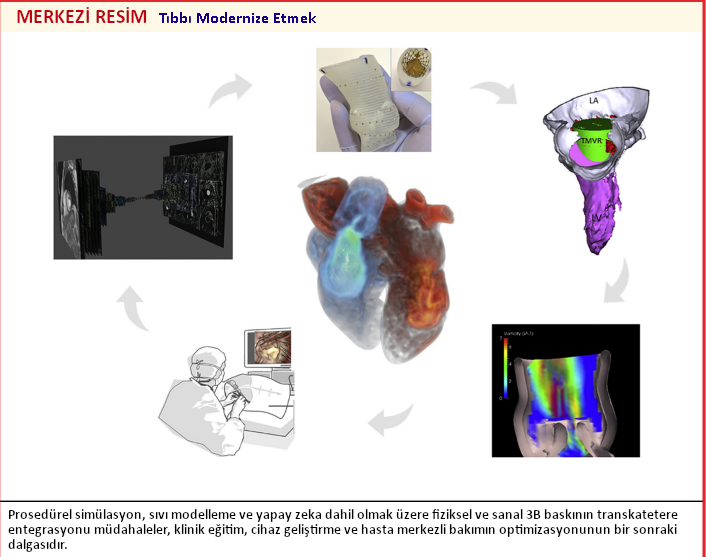
\includegraphics[width=12cm,height=8cm]{Merkezi Resim.png}
\end{block}
\end{frame}

\section{SONUÇ}

\begin{frame}{SONUÇ}

\begin{itemize}
  \item Müdahalelerde SHD içinde 3D baskı, bilgisayar simülasyonu modelleme ve derin öğrenmenin rolü vardır. 
  \item Bu teknolojilerin erken uygulanması, yeni cihaz teknolojilerinin piyasaya sürülmesiyle tanık olunan erken operatör öğrenme eğrisini azaltma potansiyeline sahiptir. 
  \item Gelecekteki hesaplamalı modelleme ve derin öğrenme uygulamaları, hasta prosedürü ve hasta veri güvenliğinin tıbbi kayıtlara ve tıbbi veri toplama paylaşım platformlarına entegrasyonunu gerektirecektir. 
  \item Multimodalite kardiyovasküler görüntülemenin geleceği, kardiyak patofizyolojinin klinik bilgisinin biyomedikal mühendislerinin teknik uzmanlığı ve bilgisayar bilimcilerinin yazılım geliştirme bilgisi ile bütünleştirilmesini gerektirecektir. 
\end{itemize}

\end{frame}

\begin{frame}{}
\begin{block}{}
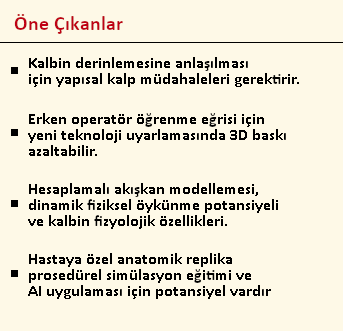
\includegraphics[width=12cm,height=8cm]{Öne Çıkanlar.png}
\end{block}
\end{frame}

\section{KAYNAK}

\begin{frame}{KAYNAK}
\begin{itemize}
\item Makale: \cite{ELSEVIER}
\bibliographystyle{plain}
\scriptsize
\bibliography{kaynak}
\end{itemize}
\end{frame}

\end{document}
